\documentclass{article}
% PACKAGES
\usepackage[english]{babel}
\usepackage{graphicx} % Required for inserting images
\usepackage[most]{tcolorbox}
\usepackage{lmodern}
\usepackage{titlepic}
\usepackage{pdfpages}
\usepackage{tcolorbox}
\usepackage{amsmath}
\usepackage{pgfplots}
\usepackage{xcolor}
\usepackage{tikz}
\usepackage{color,soul}
\usepackage{enumerate}
\usepackage{enumitem}
\usepackage{cancel}
\usepackage{hyperref} 
\usepackage{tikzsymbols}
\usepackage{fontawesome5}
\usepackage[export]{adjustbox}
\usepackage{amssymb}
\usepackage{tikz,lipsum,lmodern}
\usepackage{booktabs}


% COLOURS
\definecolor{Orchid}{RGB}{218, 112, 214}
\definecolor{snow}{rgb}{1.0, 0.98, 0.98}
\definecolor{mordantred19}{rgb}{0.68, 0.05, 0.0}
\definecolor{mistyrose}{rgb}{1.0, 0.89, 0.88}
\definecolor{nadeshikopink}{rgb}{0.96, 0.68, 0.78}
\definecolor{cadmiumgreen}{rgb}{0.0, 0.42, 0.24}
\definecolor{OliveGreen}{RGB}{85, 107, 47}
\definecolor{RoyalPurple}{RGB}{120, 81, 169}
\definecolor{NavyBlue}{RGB}{0, 0, 128}
\definecolor{CornflowerBlue}{RGB}{100, 149, 237}
\definecolor{Cerulean}{RGB}{0, 123, 167}
\definecolor{DarkOrchid}{RGB}{153, 50, 204}

\title{MCV4U - Calculus and Vectors [Chapter 3]}
\author{Kensukeken}
\date{March 8th, 2024}

\begin{document}
\maketitle

\tableofcontents
\newpage
\section{Unit 3 - Derivatives and Applications}
\subsection{Higher Order Derivatives, Velocity, Acceleration, and Rates of Change}
\subsubsection*{Second Derivative Test}
The second derivative of $y=f(x)$ is the derivative of $y=f^{\prime}(x)$\\
In Newton notation, the second derivative is $f^{\prime \prime}(x)$\\
In Leibniz notation, the second derivative is $\frac{d^2 y}{d x^2}$\\

\underline{Displacement:} The position of an object with respect to time, usually referred to as $s(t)$.\\

\underline{Velocity:} The rate of change of displacement over time. Therefore, the first derivative of the displacement function with respect to time is velocity.\\
$$
v(t)=s^{\prime}(t) \quad \text { or } \quad v(t)=\frac{d s}{d t}
$$

\underline{Acceleration:} The rate of change of velocity over time. Therefore, the first derivative of the velocity function with respect to time, or the second derivative of displacement with respect to time, is acceleration.\\
$$
a(t)=v^{\prime}(t)=s^{\prime \prime}(t) \quad \text { or } \quad a(t)=\frac{d v}{d t}=\frac{d^2 s}{d t^2}
$$

\underline{Some Points to Ponder About Velocity and Acceleration}
\begin{itemize}
\item Negative velocity means that an object is moving in a negative direction (left or down) while positive velocity means the opposite
\item Zero velocity means that an object is stationary and that a possible change in direction may occur.
\item Negative acceleration means that the velocity is decreasing, while positive acceleration means that the velocity is increasing.
\item Zero acceleration means that the velocity is constant
\item The speed of an object is the magnitude of its velocity.
$$
\text {Speed }=|v(t)|=\left|s^{\prime}(t)\right|
$$
\item An object is speeding up (increasing speed) when its velocity and acceleration have the same signs. However, an object is slowing down (decreasing speed) when its velocity and acceleration have opposite signs.
\item If the displacement is measured in metres and time is measured in seconds, then velocity is measured in $\mathrm{m} / \mathrm{s}$ and the acceleration is measured in $\mathrm{m} / \mathrm{s}^2$.
\end{itemize}



\subsubsection*{Concavity}

We know that the sign of the derivative tells us whether a function is increasing or decreasing at some point. Likewise, the sign of the second derivative $f''(x)$ tells us whether $f'(x)$ is increasing or decreasing at $x$. We summarize the consequences of this seemingly simple idea in the table below:


\begin{figure}[ht]
    \centering
    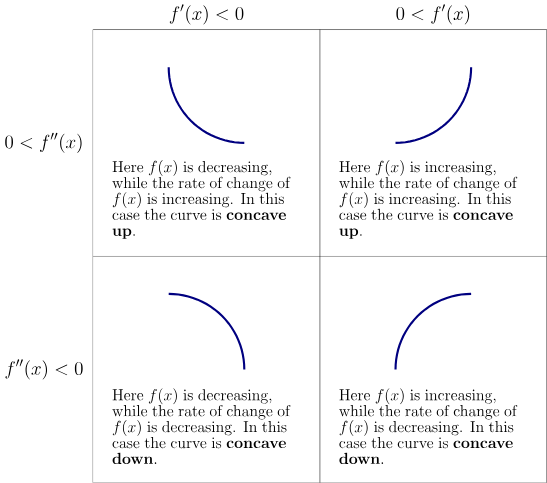
\includegraphics[width=0.7\textwidth]{imgs/digInConcavityAnd2ndDerivTest-figure0.png}
\end{figure}

The sign of the second derivative $f''(x)$ tells us about the behavior of the first derivative $f'(x)$:

\begin{center}
\begin{tabular}{@{}ll@{}}
\toprule
Sign of $f''(x)$ & Behavior of $f'(x)$ \\
\midrule
$f''(x) > 0$ & $f'(x)$ is increasing (concave up) \\
$f''(x) < 0$ & $f'(x)$ is decreasing (concave down) \\
\bottomrule
\end{tabular}
\end{center}



\newpage 

\subsubsection*{Example:}
\begin{center}
\begin{minipage}{\linewidth}
    \centering
    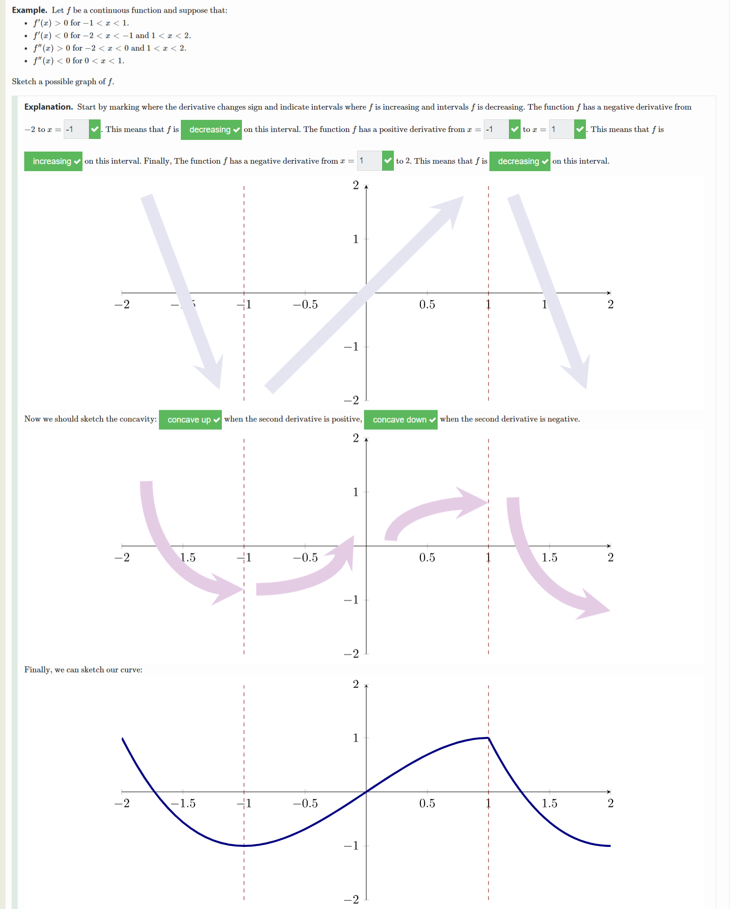
\includegraphics[width=1.3\textwidth]{imgs/ex.png}
\end{minipage}
\end{center}

\newpage 
\subsection{Inflection Points}
If we are trying to understand the shape of the graph of a function, knowing where it is concave up and concave down helps us to get a more accurate picture. Of particular interest are points at which the concavity changes from up to down or down to up.

\begin{tcolorbox}[sharp corners=uphill]
\underline{Definition:} If the concavity of $f$ changes either from up to down or down to up at $x=a$ and $f$ has a tangent line at $x=a$, then $x=a$ is an inflection point of $f$.
\end{tcolorbox}

It is instructive to see some examples of inflection points:

\begin{figure}[ht]
    \centering
    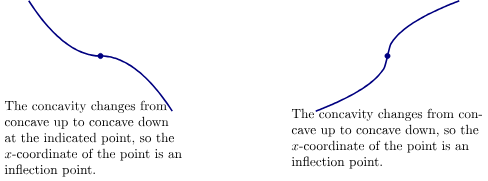
\includegraphics[width=0.7\textwidth]{imgs/digInConcavityAnd2ndDerivTest-figure4.png}
\end{figure}

\begin{figure}[ht]
    \centering
    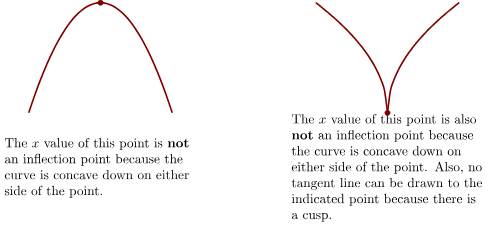
\includegraphics[width=0.7\textwidth]{imgs/digInConcavityAnd2ndDerivTest-figure5.png}
\end{figure}

\textcolor{red}{Warning:} Even if $f''(a)=0$, the point determined by $x=a$ might not be an inflection point. You also need to check that the concavity of $f$ changes on either side of $x=a$.
\newpage 

\subsubsection*{Example:}
\begin{center}
\begin{minipage}{\linewidth}
    \centering
    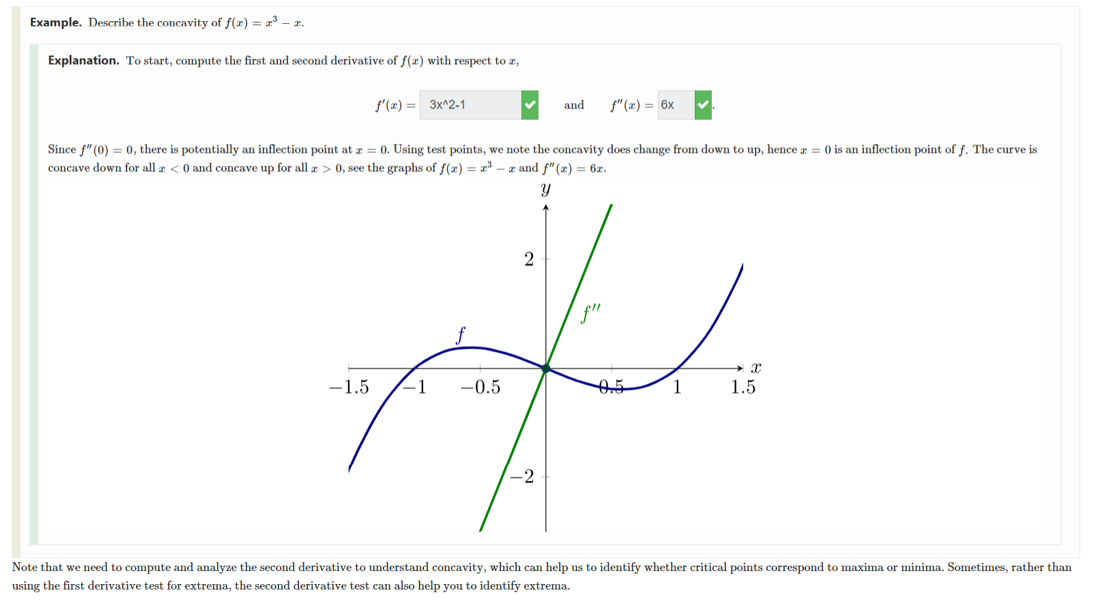
\includegraphics[width=1.3\textwidth]{imgs/ex3.png}
\end{minipage}
\end{center}
\underline{Problem:}
If $f''(a)=0$, what does the second derivative test tell us?


\begin{enumerate}
    \item[a)] The function has a local extrema at $x=a$
    \item[b)] The function does not have a local extrema at $x=a$
    \item[c)] It gives no information on whether $x=a$ is a local extremmum.
\end{enumerate}
The correct answer is C.
\subsubsection*{Example:}
\begin{center}
\begin{minipage}{\linewidth}
    \centering
    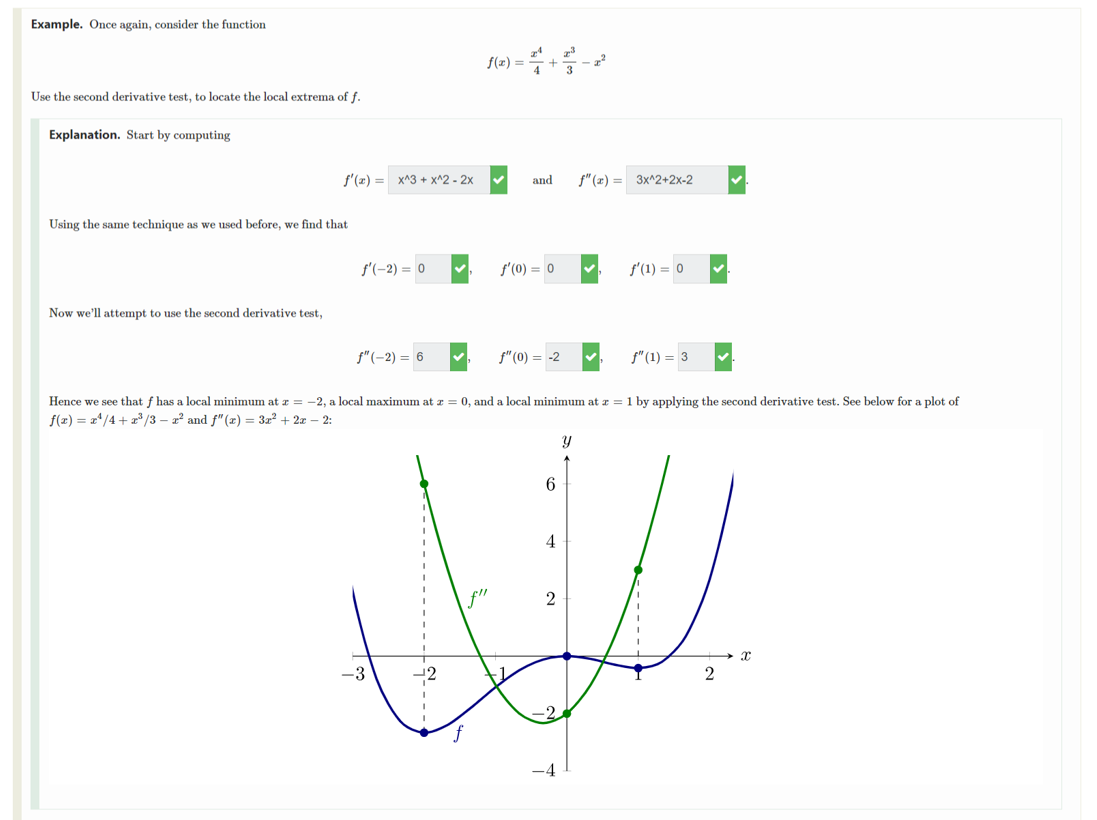
\includegraphics[width=1.3\textwidth]{imgs/ex4.png}
\end{minipage}
\end{center}
\underline{Second Derivative Test:}

\begin{itemize}
\item If $f'(c)=0$ and $f''(c)>0$, then there is a local minimum at $x=c$.
\item If $f'(c)=0$ and $f''(c)<0$, then there is a local maximum at $x=c$.
\item If $f'(c)=0$ and $f''(c)=0$, or if $f''(c)$ doesn't exist, then the test is inconclusive. There might be a local maximum or minimum, or there might be a point of inflection.
\end{itemize}
\newpage 
\subsection{Problem-Solving Strategy: Solving Optimization Problems}

\begin{enumerate}
    \item Introduce all variables. If applicable, draw a figure and label all variables.
    \item Determine which quantity is to be maximized or minimized, and for what range of values of the other variables (if this can be determined at this time).
    \item Write a formula for the quantity to be maximized or minimized in terms of the variables. This formula may involve more than one variable.
    \item Write any equations relating the independent variables in the formula from step 3. Use these equations to write the quantity to be maximized or minimized as a function of one variable.
    \item Identify the domain of consideration for the function in step 4 based on the physical problem to be solved.
    \item Locate the maximum or minimum value of the function from step 4. This step typically involves looking for critical points and evaluating a function at endpoints.
\end{enumerate}
You need to remember the surface area formulas from grade 8th math.
\begin{center}
\begin{minipage}{\linewidth}
    \centering
    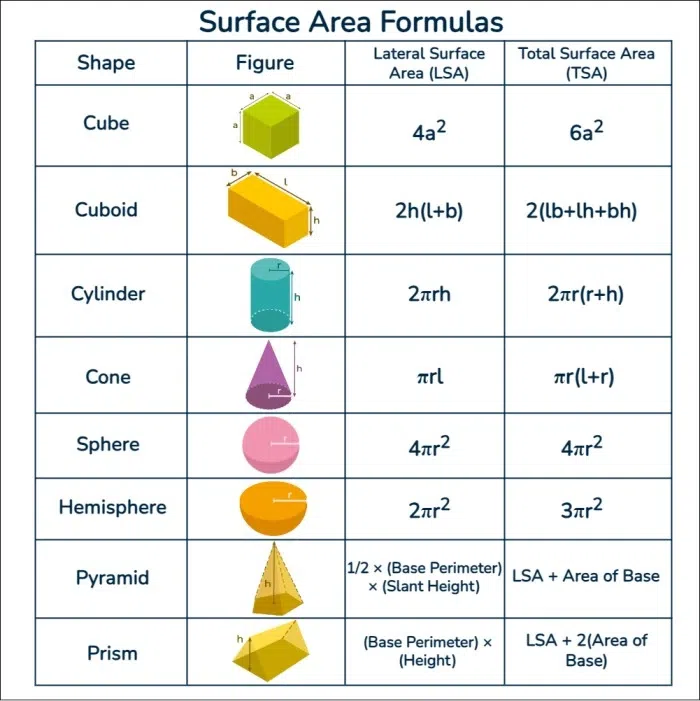
\includegraphics[width=0.8\textwidth]{imgs/Surface-Area-Formulas.png}
\end{minipage}
\end{center}
\newpage

\section*{Resources}
\begin{itemize}
    \item \href{https://explorer.globe.engineer/?q=SOLID+MENSURATION}{Solid Mensuration}
    \item \href{https://www.youtube.com/watch?v=9W4ejz0EMtE}{First Derivative Test - YouTube}
    \item \href{https://www.cuemath.com/calculus/first-derivative-test/}{First Derivative Test - Cuemath}
    \item \href{https://web.ma.utexas.edu/users/m408n/CurrentWeb/LM4-3-5.php}{The First Derivative Test - ma.utexas.edu} \& \href{https://web.ma.utexas.edu/users/m408n/AS-back-up/LM4-3-10.html}{Concavity, Points of Inflection, and the Second Derivative Test}
    \item \href{https://math.libretexts.org/Courses/University_of_California_Davis/UCD_Mat_21A%3A_Differential_Calculus/4%3A_Applications_of_Definite_Integrals/4.1%3A_Extreme_Values_of_Functions}{Local Extrema}
    \item \href{https://www.youtube.com/watch?app=desktop&v=3wrXDw5ETh4}{Finding Absolute Maximum and Minimum Values - Absolute Extrema }
    \item \href{https://www.kristakingmath.com/blog/critical-points-first-derivative-test}{Points where the derivative is either zero or undefined}
    \item \href{https://www.youtube.com/watch?app=desktop&v=P7SFDGCC3sE}{Finding critical points where undefined - YouTube}
    \item \href{https://testbook.com/maths/critical-point}{Critical Point}
    \item \href{https://www.bartleby.com/subject/math/calculus/concepts/minimization}{Maximizing or minimizing a function subject to constraints}
    \item \href{https://www.whitman.edu/mathematics/calculus_online/section06.01.html}{Optimizations}
    \item \href{https://explorer.globe.engineer/?q=important+formulas+for+optimization+in+derivatives}{Important formulas for optimization in derivatives}
    \item \href{https://openstax.org/books/calculus-volume-1/pages/4-7-applied-optimization-problems}{Optimizations problems}
\end{itemize}


\end{document}